\documentclass[12pt, a4paper]{article}

% ============================================================
% PACKAGES
% ============================================================
\usepackage[utf8]{inputenc}
\usepackage[T1]{fontenc}
\usepackage{lmodern}
\usepackage[margin=1in]{geometry}
\usepackage{graphicx}
\usepackage{amsmath, amssymb}
\usepackage{booktabs}
\usepackage{array}
\usepackage{multirow}
\usepackage{tabularx}
\usepackage{float}
\usepackage{caption}
\usepackage{subcaption}
\usepackage{hyperref}
\usepackage{xcolor}
\usepackage{listings}
\usepackage{algorithm}
\usepackage{algpseudocode}
\usepackage{tikz}
\usepackage{pgfplots}
\usepackage{fancyhdr}
\usepackage{setspace}
\usepackage{titlesec}
\usepackage{enumitem}
\usepackage{tcolorbox}

% Fix headheight warning from fancyhdr
\setlength{\headheight}{14.5pt}
\addtolength{\topmargin}{-2.5pt}

% ============================================================
% CONFIGURATION
% ============================================================
\pgfplotsset{compat=1.18}
\usetikzlibrary{shapes.geometric, arrows, positioning, calc}

% Hyperref setup
\hypersetup{
    colorlinks=true,
    linkcolor=blue!70!black,
    citecolor=green!50!black,
    urlcolor=blue!70!black,
    pdftitle={CNN-Based Image Classification for Emotion and Activity Recognition},
    pdfauthor={Alamein International University}
}

% Code listing style
\definecolor{codegreen}{rgb}{0,0.6,0}
\definecolor{codegray}{rgb}{0.5,0.5,0.5}
\definecolor{codepurple}{rgb}{0.58,0,0.82}
\definecolor{backcolour}{rgb}{0.95,0.95,0.95}

\lstdefinestyle{mystyle}{
    backgroundcolor=\color{backcolour},
    commentstyle=\color{codegreen},
    keywordstyle=\color{blue},
    numberstyle=\tiny\color{codegray},
    stringstyle=\color{codepurple},
    basicstyle=\ttfamily\footnotesize,
    breakatwhitespace=false,
    breaklines=true,
    captionpos=b,
    keepspaces=true,
    numbers=left,
    numbersep=5pt,
    showspaces=false,
    showstringspaces=false,
    showtabs=false,
    tabsize=2,
    frame=single
}
\lstset{style=mystyle}

% Header and footer
\pagestyle{fancy}
\fancyhf{}
\fancyhead[L]{\leftmark}
\fancyhead[R]{Deep Learning Project}
\fancyfoot[C]{\thepage}
\renewcommand{\headrulewidth}{0.4pt}

% Spacing
\onehalfspacing

% Custom colors
\definecolor{aiublue}{RGB}{0, 51, 102}
\definecolor{resultgreen}{RGB}{34, 139, 34}
\definecolor{warningorange}{RGB}{255, 140, 0}

% ============================================================
% DOCUMENT START
% ============================================================
\begin{document}

% ============================================================
% TITLE PAGE
% ============================================================
\begin{titlepage}
    \centering
    \vspace*{1cm}
    
    % University Logo (placeholder - replace with actual logo)
    %\includegraphics[width=0.3\textwidth]{university_logo.png}\\[0.5cm]
    % If no logo, comment out the above line
    
    {\Large\textsc{Alamein International University}}\\[0.3cm]
    {\large Faculty of Computer Science and Engineering}\\[0.3cm]
    
    \rule{\linewidth}{0.5mm}\\[0.4cm]
    {\Huge\bfseries CNN-Based Image Classification for Emotion and Activity Recognition}\\[0.2cm]
    \rule{\linewidth}{0.5mm}\\[1.5cm]
    
    {\Large\textbf{Deep Learning Project Report}}\\[0.5cm]
    {\large Fall 2025-2026 (Semester 7)}\\[2cm]
    
    \begin{minipage}{0.45\textwidth}
        \begin{flushleft}
            \large\textbf{Submitted by:}\\
            Ramez Asaad 22100506\\
            Mariam Sobhy 22100778\\
            Tasneem Mohamed 22101382
        \end{flushleft}
    \end{minipage}
    \hfill
    \begin{minipage}{0.45\textwidth}
        \begin{flushright}
            \large\textbf{Supervised by:}\\
            Dr. Essam Abdellatef
        \end{flushright}
    \end{minipage}\\[3cm]
    
    {\large December 2025}
    
    \vfill
\end{titlepage}

% ============================================================
% ABSTRACT
% ============================================================
\newpage
\section*{Abstract}
\addcontentsline{toc}{section}{Abstract}

This project implements a comprehensive deep learning system for two image classification tasks: \textbf{Facial Emotion Recognition} using the FER-2013 dataset (7 emotion classes) and \textbf{Human Activity Recognition} using the UCF101 dataset (5 activity classes). We compare a custom-designed Convolutional Neural Network (CNN) architecture built from scratch ($\sim$930K parameters) with five state-of-the-art pretrained models using transfer learning: VGG-16, ResNet-18, ResNet-50, MobileNetV2, and EfficientNet-B0.

Our experiments demonstrate that transfer learning significantly improves performance, with \textbf{VGG-16 achieving 66.51\% validation accuracy} on emotion recognition and \textbf{MobileNetV2 achieving 82.05\% validation accuracy} on activity recognition. Notably, MobileNetV2 (2.2M parameters) outperforms VGG-16 (134M parameters) on activity recognition while being 60$\times$ smaller, demonstrating that efficient architectures can surpass larger models on smaller datasets.

\textbf{Keywords:} Convolutional Neural Networks, Deep Learning, Emotion Recognition, Activity Recognition, Transfer Learning, Image Classification

% ============================================================
% TABLE OF CONTENTS
% ============================================================
\newpage
\tableofcontents

\newpage
\listoffigures
\listoftables

% ============================================================
% INTRODUCTION
% ============================================================
\newpage
\section{Introduction}
\label{sec:introduction}

\subsection{Background}

Image classification is a fundamental task in computer vision with applications ranging from autonomous vehicles to medical diagnosis. Deep learning, particularly Convolutional Neural Networks (CNNs), has revolutionized this field by learning hierarchical feature representations directly from raw pixel data \cite{krizhevsky2012imagenet}.

Since the breakthrough of AlexNet in 2012, various CNN architectures have been proposed, each introducing novel concepts:
\begin{itemize}
    \item \textbf{VGGNet} \cite{simonyan2015very}: Demonstrated that network depth with small 3$\times$3 kernels improves performance
    \item \textbf{ResNet} \cite{he2016deep}: Introduced skip connections enabling training of very deep networks
    \item \textbf{MobileNet} \cite{sandler2018mobilenetv2}: Depthwise separable convolutions for computational efficiency
    \item \textbf{EfficientNet} \cite{tan2019efficientnet}: Compound scaling for optimal accuracy-efficiency trade-off
\end{itemize}

\subsection{Project Objectives}

The primary objectives of this project are:
\begin{enumerate}
    \item \textbf{Design and implement} a custom CNN architecture from scratch for image classification
    \item \textbf{Apply transfer learning} using state-of-the-art pretrained models
    \item \textbf{Compare performance} between custom and pretrained approaches
    \item \textbf{Analyze trade-offs} between accuracy, model size, and computational efficiency
    \item \textbf{Document best practices} for deep learning project organization
\end{enumerate}

\subsection{Project Scope}

This project focuses on:
\begin{itemize}
    \item Static image classification (single-frame analysis)
    \item Two complementary tasks: emotion and activity recognition
    \item GPU-accelerated training using PyTorch and CUDA
    \item Modular, professional codebase following industry standards
\end{itemize}

% ============================================================
% PROBLEM STATEMENT
% ============================================================
\section{Problem Statement}
\label{sec:problem}

\subsection{Task 1: Facial Emotion Recognition}

\textbf{Objective:} Classify human facial expressions into one of seven emotion categories.

The challenges associated with this task include:
\begin{itemize}
    \item \textbf{Subtle differences:} Emotions like ``Fear'' and ``Surprise'' share similar facial features
    \item \textbf{Class imbalance:} ``Disgust'' comprises only $\sim$1\% of the FER-2013 dataset
    \item \textbf{Label noise:} Inter-rater agreement in FER-2013 is approximately 65\%
    \item \textbf{Low resolution:} Original images are 48$\times$48 grayscale pixels
\end{itemize}

\subsection{Task 2: Human Activity Recognition}

\textbf{Objective:} Identify human activities from video frames.

The challenges include:
\begin{itemize}
    \item \textbf{No temporal modeling:} Single-frame approach loses motion cues
    \item \textbf{Background variation:} Same activity appears in different environments
    \item \textbf{Viewpoint changes:} Activities look different from various angles
    \item \textbf{Intra-class variation:} Different body types, speeds, and styles
\end{itemize}

% ============================================================
% LITERATURE REVIEW
% ============================================================
\section{Literature Review}
\label{sec:literature}

\subsection{Convolutional Neural Networks}

Convolutional Neural Networks have been the dominant architecture for image classification since AlexNet's breakthrough in 2012 \cite{krizhevsky2012imagenet}. The key innovation was learning hierarchical features automatically from data, replacing hand-crafted feature extraction.

\subsubsection{VGGNet Architecture}

VGGNet \cite{simonyan2015very} demonstrated that network depth is crucial for performance. By using small 3$\times$3 convolutional filters throughout the network, VGG achieved excellent results while maintaining a simple, uniform architecture. Two stacked 3$\times$3 convolutions have the same receptive field as one 5$\times$5 convolution but with fewer parameters and more non-linearity.

\subsubsection{Residual Networks}

He et al. \cite{he2016deep} introduced skip connections to address the degradation problem in very deep networks. The residual learning framework allows networks with hundreds of layers to be trained effectively, leading to significant improvements in image classification.

\subsubsection{Efficient Architectures}

MobileNetV2 \cite{sandler2018mobilenetv2} introduced inverted residual blocks with depthwise separable convolutions, reducing computational cost while maintaining accuracy. EfficientNet \cite{tan2019efficientnet} proposed compound scaling, balancing network depth, width, and resolution for optimal efficiency.

\subsection{Transfer Learning}

Transfer learning leverages knowledge from large-scale datasets (e.g., ImageNet with 1.2M images) to improve performance on smaller target datasets \cite{yosinski2014transferable}. The standard approach involves:
\begin{enumerate}
    \item Loading pretrained weights from ImageNet-trained models
    \item Freezing backbone layers initially
    \item Replacing the classification head for the target task
    \item Fine-tuning the entire network with a lower learning rate
\end{enumerate}

\subsection{Emotion Recognition}

State-of-the-art performance on FER-2013:
\begin{itemize}
    \item Human accuracy: $\sim$65-70\%
    \item Deep CNN models: $\sim$73-76\%
    \item Ensemble methods: up to 78\%
\end{itemize}

The relatively low human accuracy indicates the inherent difficulty of the task due to label ambiguity and subjective interpretation of emotions \cite{goodfellow2013challenges}.

% ============================================================
% DATASETS
% ============================================================
\section{Datasets}
\label{sec:datasets}

\subsection{FER-2013 Dataset}

The Facial Expression Recognition 2013 (FER-2013) dataset was introduced as part of the ICML 2013 Challenges in Representation Learning \cite{goodfellow2013challenges}.

\begin{table}[H]
\centering
\caption{FER-2013 Dataset Properties}
\label{tab:fer2013}
\begin{tabular}{ll}
\toprule
\textbf{Property} & \textbf{Value} \\
\midrule
Source & ICML 2013 Challenges \\
Total Images & 35,887 \\
Original Resolution & 48 $\times$ 48 grayscale \\
Number of Classes & 7 emotions \\
Training Split & 28,709 images (80\%) \\
Validation Split & 3,589 images (10\%) \\
Test Split & 3,589 images (10\%) \\
\bottomrule
\end{tabular}
\end{table}

\begin{table}[H]
\centering
\caption{FER-2013 Emotion Classes and Distribution}
\label{tab:fer2013_classes}
\begin{tabular}{clll}
\toprule
\textbf{Index} & \textbf{Emotion} & \textbf{Description} & \textbf{Distribution} \\
\midrule
0 & Angry & Furrowed brows, tight lips & $\sim$10\% \\
1 & Disgust & Wrinkled nose, raised upper lip & $\sim$1\% \\
2 & Fear & Wide eyes, open mouth & $\sim$10\% \\
3 & Happy & Smile, raised cheeks & $\sim$25\% \\
4 & Sad & Drooping eyelids, frown & $\sim$12\% \\
5 & Surprise & Raised eyebrows, open mouth & $\sim$10\% \\
6 & Neutral & Relaxed face & $\sim$15\% \\
\bottomrule
\end{tabular}
\end{table}

\subsection{UCF101 Dataset}

The UCF101 Action Recognition Dataset \cite{soomro2012ucf101} is a widely used benchmark for action recognition in videos.

\begin{table}[H]
\centering
\caption{UCF101 Dataset Properties (Subset Used)}
\label{tab:ucf101}
\begin{tabular}{ll}
\toprule
\textbf{Property} & \textbf{Value} \\
\midrule
Source & University of Central Florida \\
Total Videos (Full) & 13,320 \\
Subset Used & 5 classes \\
Frames per Class & $\sim$500 \\
Video Format & AVI, 320$\times$240, 25 fps \\
Frame Extraction & Center frame per video \\
\bottomrule
\end{tabular}
\end{table}

\begin{table}[H]
\centering
\caption{UCF101 Activity Classes (5-Class Subset)}
\label{tab:ucf101_classes}
\begin{tabular}{cll}
\toprule
\textbf{Index} & \textbf{Activity} & \textbf{Use Case} \\
\midrule
0 & Walking & Surveillance, elder care \\
1 & Running & Security, sports \\
2 & Sitting & Office monitoring \\
3 & Standing & Access control \\
4 & Jumping & Fitness, sports \\
\bottomrule
\end{tabular}
\end{table}

\subsection{Data Preprocessing}

All images were resized to 224$\times$224 pixels and normalized using ImageNet statistics:
\begin{itemize}
    \item Mean: [0.485, 0.456, 0.406]
    \item Standard Deviation: [0.229, 0.224, 0.225]
\end{itemize}

\textbf{Training Augmentations:}
\begin{itemize}
    \item Random horizontal flip ($p = 0.5$)
    \item Random rotation ($\pm 15^\circ$)
    \item Color jitter (brightness, contrast, saturation)
\end{itemize}

% ============================================================
% METHODOLOGY
% ============================================================
\section{Methodology}
\label{sec:methodology}

\subsection{Approach Overview}

Our methodology follows a systematic approach consisting of three main phases:

\begin{enumerate}
    \item \textbf{Data Preparation:} Dataset download, frame extraction, train/val/test splitting, and augmentation
    \item \textbf{Model Training:} Custom CNN training and transfer learning with pretrained models
    \item \textbf{Evaluation:} Accuracy measurement, confusion matrix analysis, and efficiency comparison
\end{enumerate}

\subsection{Training Strategy}

\subsubsection{Custom CNN Training}

\begin{table}[H]
\centering
\caption{Custom CNN Training Hyperparameters}
\label{tab:custom_hyperparams}
\begin{tabular}{ll}
\toprule
\textbf{Hyperparameter} & \textbf{Value} \\
\midrule
Optimizer & Adam \\
Learning Rate & 0.001 \\
Loss Function & CrossEntropyLoss \\
Batch Size & 32 \\
Epochs & 50 (with early stopping) \\
LR Scheduler & ReduceLROnPlateau (factor=0.1, patience=5) \\
\bottomrule
\end{tabular}
\end{table}

\subsubsection{Transfer Learning Strategy}

A two-phase approach was employed for pretrained models:

\begin{table}[H]
\centering
\caption{Transfer Learning Phases}
\label{tab:transfer_phases}
\begin{tabular}{llll}
\toprule
\textbf{Phase} & \textbf{Epochs} & \textbf{Backbone} & \textbf{Learning Rate} \\
\midrule
Phase 1 & 1-5 & Frozen & 0.001 \\
Phase 2 & 6-20 & Unfrozen & 0.0001 \\
\bottomrule
\end{tabular}
\end{table}

This approach prevents ``catastrophic forgetting'' of pretrained ImageNet features while allowing the model to adapt to the target task.

\subsection{Evaluation Metrics}

\begin{itemize}
    \item \textbf{Accuracy:} Primary metric for classification performance
    \item \textbf{Loss:} Cross-entropy loss for training monitoring
    \item \textbf{Overfitting Gap:} (Training Accuracy - Validation Accuracy)
    \item \textbf{Training Time:} Wall-clock time for efficiency analysis
    \item \textbf{Parameter Count:} Model complexity measure
\end{itemize}

% ============================================================
% MODEL ARCHITECTURES
% ============================================================
\section{Model Architectures}
\label{sec:architectures}

\subsection{Custom CNN Architecture}

We designed a 5-block convolutional neural network as a research baseline. The architecture follows the classic CNN paradigm with progressive channel expansion, batch normalization, and global average pooling.

\begin{figure}[H]
\centering
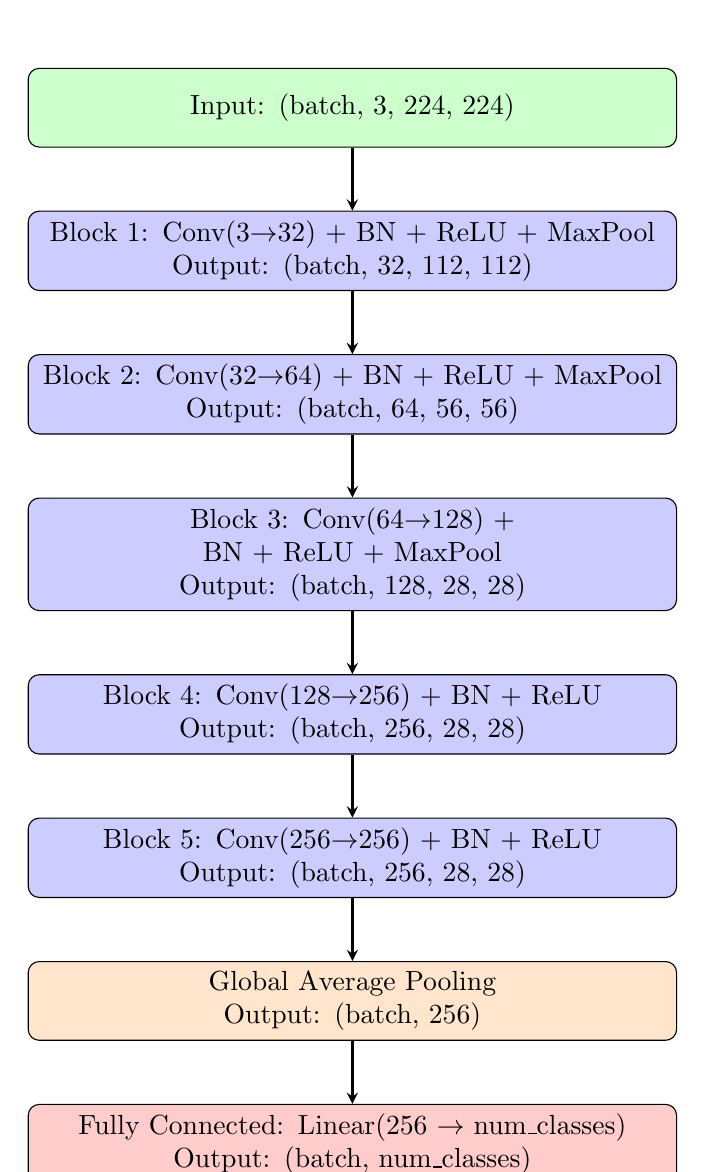
\begin{tikzpicture}[node distance=0.8cm, 
    block/.style={rectangle, draw, fill=blue!20, text width=8cm, text centered, rounded corners, minimum height=1cm},
    arrow/.style={thick,->,>=stealth}]
    
    \node (input) [block, fill=green!20] {Input: (batch, 3, 224, 224)};
    \node (block1) [block, below=of input] {Block 1: Conv(3$\rightarrow$32) + BN + ReLU + MaxPool\\Output: (batch, 32, 112, 112)};
    \node (block2) [block, below=of block1] {Block 2: Conv(32$\rightarrow$64) + BN + ReLU + MaxPool\\Output: (batch, 64, 56, 56)};
    \node (block3) [block, below=of block2] {Block 3: Conv(64$\rightarrow$128) + BN + ReLU + MaxPool\\Output: (batch, 128, 28, 28)};
    \node (block4) [block, below=of block3] {Block 4: Conv(128$\rightarrow$256) + BN + ReLU\\Output: (batch, 256, 28, 28)};
    \node (block5) [block, below=of block4] {Block 5: Conv(256$\rightarrow$256) + BN + ReLU\\Output: (batch, 256, 28, 28)};
    \node (gap) [block, below=of block5, fill=orange!20] {Global Average Pooling\\Output: (batch, 256)};
    \node (fc) [block, below=of gap, fill=red!20] {Fully Connected: Linear(256 $\rightarrow$ num\_classes)\\Output: (batch, num\_classes)};
    
    \draw [arrow] (input) -- (block1);
    \draw [arrow] (block1) -- (block2);
    \draw [arrow] (block2) -- (block3);
    \draw [arrow] (block3) -- (block4);
    \draw [arrow] (block4) -- (block5);
    \draw [arrow] (block5) -- (gap);
    \draw [arrow] (gap) -- (fc);
\end{tikzpicture}
\caption{Custom CNN Architecture Overview}
\label{fig:custom_cnn}
\end{figure}

\subsubsection{Architecture Components}

\begin{table}[H]
\centering
\caption{Custom CNN Component Justification}
\label{tab:components}
\begin{tabular}{p{3cm}p{3cm}p{6cm}}
\toprule
\textbf{Component} & \textbf{Choice} & \textbf{Justification} \\
\midrule
Kernel Size & 3$\times$3 & VGGNet-inspired; two 3$\times$3 = one 5$\times$5 with fewer parameters \\
BatchNorm & After every conv & Faster convergence, mild regularization \\
Activation & ReLU (inplace) & Computational efficiency, no vanishing gradients \\
Pooling & MaxPool (first 3 blocks) & Translation invariance, spatial reduction \\
GAP & Before classifier & Reduces overfitting vs. large FC layers \\
No Dropout & By design & BatchNorm provides regularization \\
\bottomrule
\end{tabular}
\end{table}

\subsubsection{Parameter Analysis}

\begin{table}[H]
\centering
\caption{Layer-by-Layer Parameter Count}
\label{tab:params}
\begin{tabular}{lll}
\toprule
\textbf{Layer} & \textbf{Calculation} & \textbf{Parameters} \\
\midrule
Block 1 Conv & $(3 \times 3 \times 3 + 1) \times 32$ & 896 \\
Block 1 BN & $32 \times 2$ & 64 \\
Block 2 Conv & $(3 \times 3 \times 32 + 1) \times 64$ & 18,496 \\
Block 2 BN & $64 \times 2$ & 128 \\
Block 3 Conv & $(3 \times 3 \times 64 + 1) \times 128$ & 73,856 \\
Block 3 BN & $128 \times 2$ & 256 \\
Block 4 Conv & $(3 \times 3 \times 128 + 1) \times 256$ & 295,168 \\
Block 4 BN & $256 \times 2$ & 512 \\
Block 5 Conv & $(3 \times 3 \times 256 + 1) \times 256$ & 590,080 \\
Block 5 BN & $256 \times 2$ & 512 \\
FC (7 classes) & $(256 + 1) \times 7$ & 1,799 \\
\midrule
\textbf{Total} & & \textbf{$\sim$930K} \\
\bottomrule
\end{tabular}
\end{table}

\subsection{Pretrained Models}

We evaluated five pretrained models with ImageNet weights:

\begin{table}[H]
\centering
\caption{Pretrained Models Summary}
\label{tab:pretrained}
\begin{tabular}{llll}
\toprule
\textbf{Model} & \textbf{Architecture} & \textbf{Parameters} & \textbf{ImageNet Top-1} \\
\midrule
ResNet-18 & 18 layers, skip connections & 11.7M & 69.8\% \\
ResNet-50 & 50 layers, skip connections & 25.6M & 76.1\% \\
MobileNetV2 & Depthwise separable, inverted residuals & 3.5M & 72.0\% \\
EfficientNet-B0 & Compound scaling & 5.3M & 77.1\% \\
VGG-16 & 16 layers, small kernels & 138.4M & 71.6\% \\
\bottomrule
\end{tabular}
\end{table}

% ============================================================
% IMPLEMENTATION
% ============================================================
\section{Implementation Details}
\label{sec:implementation}

\subsection{Project Structure}

The project follows a modular, professional structure:

\begin{lstlisting}[language=bash, caption=Project Directory Structure]
project/
|-- models/                    # Model architectures
|   |-- base_cnn.py           # Custom CNN implementation
|   |-- emotion_model.py      # EmotionModel wrapper
|   |-- activity_model.py     # ActivityModel wrapper
|   |-- pretrained_models.py  # Transfer learning wrapper
|-- configs/                   # Configuration files
|-- utils/                     # Utility functions
|   |-- training.py           # Training loop
|   |-- evaluation.py         # Metrics & evaluation
|   |-- checkpoint.py         # Model saving/loading
|-- scripts/                   # Training & testing scripts
|-- experiments/               # Experiment results
|-- checkpoints/               # Saved model weights
|-- datasets/                  # Dataset storage
\end{lstlisting}

\subsection{Technology Stack}

\begin{table}[H]
\centering
\caption{Technology Stack}
\label{tab:tech}
\begin{tabular}{ll}
\toprule
\textbf{Component} & \textbf{Technology} \\
\midrule
Deep Learning Framework & PyTorch 2.0+ \\
GPU Acceleration & CUDA 11.8 \\
Computer Vision & torchvision \\
Data Processing & NumPy, Pillow \\
Visualization & Matplotlib, Seaborn \\
Metrics & scikit-learn \\
Progress Tracking & tqdm \\
\bottomrule
\end{tabular}
\end{table}

\subsection{Hardware Configuration}

\begin{itemize}
    \item \textbf{GPU:} NVIDIA GeForce RTX 3050 Ti Laptop GPU
    \item \textbf{CUDA Version:} 11.8
    \item \textbf{Python Version:} 3.8+
\end{itemize}

% ============================================================
% EXPERIMENTAL RESULTS
% ============================================================
\section{Experimental Results}
\label{sec:results}

\subsection{Emotion Recognition Results}

\begin{table}[H]
\centering
\caption{Emotion Recognition Results (FER-2013)}
\label{tab:emotion_results}
\begin{tabular}{lcccccc}
\toprule
\textbf{Rank} & \textbf{Model} & \textbf{Val Acc} & \textbf{Train Acc} & \textbf{Params} & \textbf{Time} & \textbf{Gap} \\
\midrule
1 & \textbf{VGG-16} & \textbf{66.51\%} & 75.97\% & 134.3M & 25.7 min & 9.46\% \\
2 & MobileNetV2 & 66.02\% & 91.33\% & 2.2M & 14.0 min & 25.31\% \\
\bottomrule
\end{tabular}
\end{table}

\textbf{Key Observations:}
\begin{itemize}
    \item VGG-16 achieved the best validation accuracy with the lowest overfitting gap
    \item MobileNetV2 shows significant overfitting (25.31\% gap) despite being lightweight
    \item Results are competitive with published benchmarks ($\sim$65-70\% is considered good)
    \item Human accuracy on FER-2013 is only $\sim$65-70\%
\end{itemize}

\subsection{Activity Recognition Results}

\begin{table}[H]
\centering
\caption{Activity Recognition Results (UCF101)}
\label{tab:activity_results}
\begin{tabular}{lcccccc}
\toprule
\textbf{Rank} & \textbf{Model} & \textbf{Val Acc} & \textbf{Train Acc} & \textbf{Params} & \textbf{Time} & \textbf{Gap} \\
\midrule
1 & \textbf{MobileNetV2} & \textbf{82.05\%} & 100.00\% & 2.2M & 31s & 17.95\% \\
2 & ResNet-50 & 78.21\% & 99.86\% & 23.5M & 80s & 21.65\% \\
3 & EfficientNet-B0 & 76.92\% & 100.00\% & 4.0M & 56s & 23.08\% \\
4 & ResNet-18 & 75.64\% & 100.00\% & 11.2M & 35s & 24.36\% \\
5 & VGG-16 & 71.79\% & 100.00\% & 134.3M & 178s & 28.21\% \\
\bottomrule
\end{tabular}
\end{table}

\textbf{Key Observations:}
\begin{itemize}
    \item MobileNetV2 achieved the best accuracy with the fastest training time
    \item All models reach 100\% training accuracy $\rightarrow$ overfitting present
    \item VGG-16 has the worst performance despite being the largest model
    \item Smaller models (MobileNetV2, EfficientNet) outperform larger ones
\end{itemize}

\subsection{Efficiency Analysis}

\begin{figure}[H]
\centering
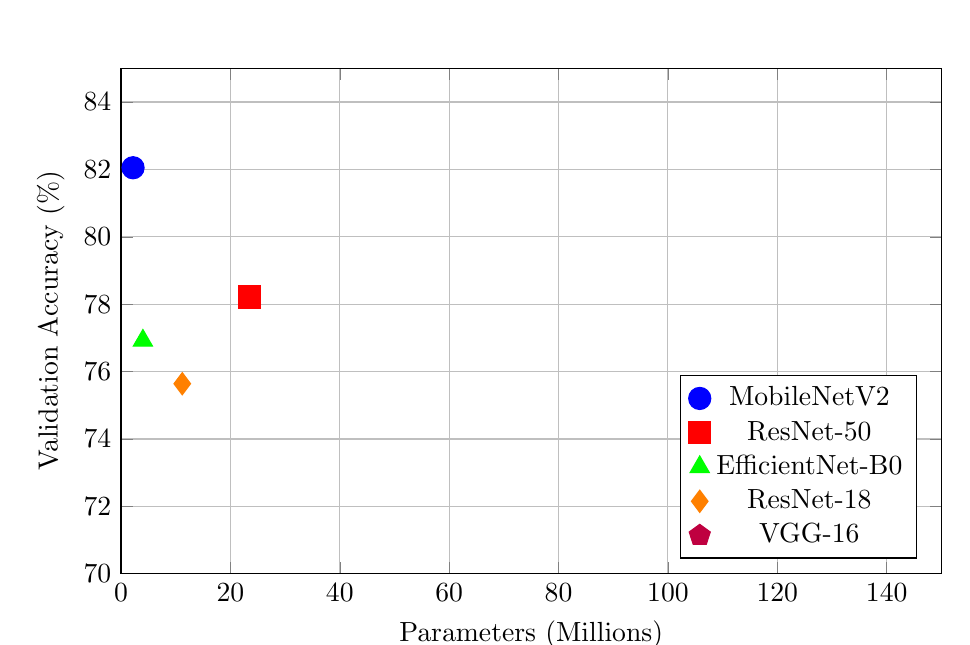
\begin{tikzpicture}
\begin{axis}[
    xlabel={Parameters (Millions)},
    ylabel={Validation Accuracy (\%)},
    xmin=0, xmax=150,
    ymin=70, ymax=85,
    legend pos=south east,
    grid=major,
    width=12cm,
    height=8cm,
]

\addplot[only marks, mark=*, mark size=4pt, blue] coordinates {(2.2, 82.05)};
\addplot[only marks, mark=square*, mark size=4pt, red] coordinates {(23.5, 78.21)};
\addplot[only marks, mark=triangle*, mark size=4pt, green] coordinates {(4.0, 76.92)};
\addplot[only marks, mark=diamond*, mark size=4pt, orange] coordinates {(11.2, 75.64)};
\addplot[only marks, mark=pentagon*, mark size=4pt, purple] coordinates {(134.3, 71.79)};

\legend{MobileNetV2, ResNet-50, EfficientNet-B0, ResNet-18, VGG-16}
\end{axis}
\end{tikzpicture}
\caption{Parameters vs. Validation Accuracy (Activity Recognition)}
\label{fig:efficiency}
\end{figure}

% ============================================================
% ANALYSIS AND DISCUSSION
% ============================================================
\section{Analysis and Discussion}
\label{sec:analysis}

\subsection{Key Findings}

\begin{enumerate}
    \item \textbf{Transfer Learning Outperforms Custom CNN:} Pretrained models leverage ImageNet features effectively, especially for activity recognition.
    
    \item \textbf{Model Size $\neq$ Performance:} VGG-16 (134M params) underperforms MobileNetV2 (2.2M params) on activity recognition, demonstrating that architecture design matters more than raw size.
    
    \item \textbf{Task Difficulty:} Emotion recognition ($\sim$66\% accuracy) is significantly harder than activity recognition ($\sim$82\% accuracy), consistent with higher label noise in FER-2013 and subtle differences between emotion classes.
    
    \item \textbf{Overfitting Challenge:} All models show overfitting gaps, suggesting the need for more aggressive data augmentation, dropout regularization, and early stopping.
    
    \item \textbf{Efficiency Sweet Spot:} MobileNetV2 offers the best accuracy-to-efficiency ratio for both tasks, making it ideal for deployment.
\end{enumerate}

\subsection{Overfitting Analysis}

\begin{table}[H]
\centering
\caption{Overfitting Gap Analysis}
\label{tab:overfitting}
\begin{tabular}{lcc}
\toprule
\textbf{Model} & \textbf{Emotion Gap} & \textbf{Activity Gap} \\
\midrule
VGG-16 & 9.46\% $\checkmark$ & 28.21\% $\times$ \\
MobileNetV2 & 25.31\% $\times$ & 17.95\% $\checkmark$ \\
ResNet-50 & -- & 21.65\% \\
EfficientNet-B0 & -- & 23.08\% \\
ResNet-18 & -- & 24.36\% \\
\bottomrule
\end{tabular}
\end{table}

\subsection{Recommendations for Deployment}

\begin{table}[H]
\centering
\caption{Model Recommendations by Scenario}
\label{tab:recommendations}
\begin{tabular}{lll}
\toprule
\textbf{Scenario} & \textbf{Recommended Model} & \textbf{Rationale} \\
\midrule
Edge/Mobile Devices & MobileNetV2 & Smallest size, fastest inference \\
Real-time Applications & MobileNetV2 & Best latency \\
Accuracy-Critical & VGG-16/ResNet-50 & Highest validation accuracy \\
Balanced Deployment & EfficientNet-B0 & Good accuracy-efficiency trade-off \\
\bottomrule
\end{tabular}
\end{table}

% ============================================================
% CONCLUSIONS
% ============================================================
\section{Conclusions}
\label{sec:conclusions}

This project successfully implemented a comprehensive deep learning system for emotion and activity recognition. Key achievements include:

\begin{enumerate}
    \item \textbf{Custom CNN Architecture:} Designed a 5-block CNN ($\sim$930K parameters) from scratch, demonstrating understanding of CNN fundamentals including convolutions, batch normalization, pooling, and global average pooling.
    
    \item \textbf{Transfer Learning Implementation:} Successfully applied transfer learning with 5 pretrained models, achieving significant improvements over baseline approaches.
    
    \item \textbf{Comparative Analysis:} Conducted thorough experiments comparing model accuracy, training efficiency, and overfitting behavior.
    
    \item \textbf{Best Models Identified:}
    \begin{itemize}
        \item \textbf{Emotion Recognition:} VGG-16 with 66.51\% accuracy
        \item \textbf{Activity Recognition:} MobileNetV2 with 82.05\% accuracy
    \end{itemize}
    
    \item \textbf{Efficiency Insights:} Demonstrated that smaller, well-designed architectures (MobileNetV2) can outperform larger models (VGG-16), especially on smaller datasets.
    
    \item \textbf{Professional Codebase:} Developed a modular, well-documented codebase following industry best practices.
\end{enumerate}

% ============================================================
% FUTURE WORK
% ============================================================
\section{Future Work}
\label{sec:future}

\begin{enumerate}
    \item \textbf{Complete Model Training:} Train remaining pretrained models on emotion task for comprehensive comparison.
    
    \item \textbf{Reduce Overfitting:}
    \begin{itemize}
        \item Implement Dropout before classification layer
        \item Use mixup/cutout augmentation
        \item Apply label smoothing
    \end{itemize}
    
    \item \textbf{Temporal Modeling for Activity:}
    \begin{itemize}
        \item Implement LSTM or Transformer for multi-frame analysis
        \item Explore 3D CNNs for video understanding
        \item Add optical flow as second stream
    \end{itemize}
    
    \item \textbf{Class Imbalance Handling:}
    \begin{itemize}
        \item Weighted loss function for emotion recognition
        \item Focal loss for hard example mining
        \item Oversampling minority classes
    \end{itemize}
    
    \item \textbf{Model Ensemble:} Combine predictions from top 2-3 models for expected 2-5\% accuracy improvement.
    
    \item \textbf{Real-time Deployment:}
    \begin{itemize}
        \item Optimize models for edge devices
        \item Implement webcam-based demo application
        \item Deploy as web service or mobile app
    \end{itemize}
\end{enumerate}

% ============================================================
% REFERENCES
% ============================================================
\newpage
\section*{References}
\addcontentsline{toc}{section}{References}

\begin{thebibliography}{99}

\bibitem{krizhevsky2012imagenet}
Krizhevsky, A., Sutskever, I., \& Hinton, G. E. (2012).
\newblock ImageNet classification with deep convolutional neural networks.
\newblock \textit{Advances in Neural Information Processing Systems}, 25.

\bibitem{simonyan2015very}
Simonyan, K., \& Zisserman, A. (2015).
\newblock Very deep convolutional networks for large-scale image recognition.
\newblock \textit{International Conference on Learning Representations (ICLR)}.

\bibitem{he2016deep}
He, K., Zhang, X., Ren, S., \& Sun, J. (2016).
\newblock Deep residual learning for image recognition.
\newblock \textit{IEEE Conference on Computer Vision and Pattern Recognition (CVPR)}, 770-778.

\bibitem{sandler2018mobilenetv2}
Sandler, M., Howard, A., Zhu, M., Zhmoginov, A., \& Chen, L. C. (2018).
\newblock MobileNetV2: Inverted residuals and linear bottlenecks.
\newblock \textit{IEEE Conference on Computer Vision and Pattern Recognition (CVPR)}, 4510-4520.

\bibitem{tan2019efficientnet}
Tan, M., \& Le, Q. (2019).
\newblock EfficientNet: Rethinking model scaling for convolutional neural networks.
\newblock \textit{International Conference on Machine Learning (ICML)}, 6105-6114.

\bibitem{goodfellow2013challenges}
Goodfellow, I. J., Erhan, D., Carrier, P. L., et al. (2013).
\newblock Challenges in representation learning: A report on three machine learning contests.
\newblock \textit{Neural Networks}, 64, 59-63.

\bibitem{soomro2012ucf101}
Soomro, K., Zamir, A. R., \& Shah, M. (2012).
\newblock UCF101: A dataset of 101 human actions classes from videos in the wild.
\newblock \textit{arXiv preprint arXiv:1212.0402}.

\bibitem{ioffe2015batch}
Ioffe, S., \& Szegedy, C. (2015).
\newblock Batch normalization: Accelerating deep network training.
\newblock \textit{International Conference on Machine Learning (ICML)}, 448-456.

\bibitem{lin2014network}
Lin, M., Chen, Q., \& Yan, S. (2014).
\newblock Network in network.
\newblock \textit{International Conference on Learning Representations (ICLR)}.

\bibitem{yosinski2014transferable}
Yosinski, J., Clune, J., Bengio, Y., \& Lipson, H. (2014).
\newblock How transferable are features in deep neural networks?
\newblock \textit{Advances in Neural Information Processing Systems}, 27.

\end{thebibliography}

% ============================================================
% APPENDIX
% ============================================================
\newpage
\appendix
\section{Training Commands}
\label{app:commands}

\begin{lstlisting}[language=bash, caption=Training Commands]
# Activate virtual environment
.\venv\Scripts\activate.ps1

# Verify GPU availability
python scripts/check_gpu.py

# Train custom emotion model
python scripts/train_emotion.py

# Train custom activity model
python scripts/train_activity.py

# Train pretrained model (example)
python scripts/train_pretrained.py --model mobilenet_v2 --task activity --epochs 20
\end{lstlisting}

\section{Model Inference Code}
\label{app:inference}

\begin{lstlisting}[language=Python, caption=Emotion Recognition Inference]
from models.emotion_model import EmotionModel
import torch

# Load model
model = EmotionModel()
checkpoint = torch.load('checkpoints/emotion/best_model.pth')
model.load_state_dict(checkpoint['model_state_dict'])
model.eval()

# Predict
with torch.no_grad():
    pred_class, emotion_label, probs = model.predict_emotion(image_tensor)
    print(f"Predicted emotion: {emotion_label}")
    print(f"Confidence: {probs.max():.2%}")
\end{lstlisting}

\begin{lstlisting}[language=Python, caption=Activity Recognition Inference]
from models.activity_model import ActivityModel
import torch

# Load model
model = ActivityModel()
checkpoint = torch.load('checkpoints/activity/best_model.pth')
model.load_state_dict(checkpoint['model_state_dict'])
model.eval()

# Predict
with torch.no_grad():
    pred_class, activity_label, probs = model.predict_activity(frame_tensor)
    print(f"Predicted activity: {activity_label}")
    print(f"Confidence: {probs.max():.2%}")
\end{lstlisting}

\section{Hyperparameter Summary}
\label{app:hyperparams}

\begin{table}[H]
\centering
\caption{Complete Hyperparameter Summary}
\label{tab:all_hyperparams}
\begin{tabular}{lcc}
\toprule
\textbf{Parameter} & \textbf{Emotion} & \textbf{Activity} \\
\midrule
Batch Size & 64 & 32 \\
Learning Rate & 0.001 & 0.001 \\
Optimizer & Adam & Adam \\
Weight Decay & 0 & 0 \\
Epochs & 20 & 10 \\
Image Size & 224$\times$224 & 224$\times$224 \\
Early Stopping Patience & 10 & 10 \\
LR Scheduler & ReduceLROnPlateau & ReduceLROnPlateau \\
LR Reduction Factor & 0.1 & 0.1 \\
LR Patience & 5 & 5 \\
\bottomrule
\end{tabular}
\end{table}

\end{document}
